\documentclass[conference]{IEEEtran}

\usepackage{amsmath}
\usepackage{amssymb}
\usepackage{booktabs}
\usepackage{cite}
\usepackage{graphicx}
\usepackage{url}
\usepackage{xurl}
\usepackage{tikz}
\usetikzlibrary{arrows.meta,positioning}
\usepackage[hidelinks]{hyperref}

\graphicspath{{figures/}}

\begin{document}

\title{A Sonar-Inspired Acoustic OFDM Testbed for Reproducible Multipath Packet-Recovery Experiments}

\author{
\IEEEauthorblockN{Giancarla Burgos}
\IEEEauthorblockA{ES 156 Final Project}
}

\maketitle

\begin{abstract}
This project studies when cyclic-prefix OFDM turns a dispersive multipath channel into separate frequency bins that can be corrected independently, and what robustness/rate tradeoff that requires. The system is a reproducible acoustic-OFDM testbed for reverberant room-acoustic and sonar-inspired links, not a finished underwater communication system. The baseline is single-carrier pulse-amplitude modulation (PAM) with a matched-filter receiver, which makes intersymbol interference visible.  The main system is orthogonal frequency-division multiplexing (OFDM), where an inverse DFT creates parallel subcarriers and a cyclic prefix converts channel convolution into an approximately circular convolution.  After cyclic-prefix removal, the received subcarrier values satisfy the scalar model $Y[k]=H[k]X[k]+W[k]$, enabling one-tap FFT-domain equalization.  Reproducible simulations compare matched filtering, OFDM without equalization, OFDM without a cyclic prefix, OFDM with perfect channel knowledge, and OFDM with a training-symbol channel estimate.  A Monte Carlo BER sweep, a cyclic-prefix-length sweep, and constellation plots show both the benefit and the cost of the cyclic prefix.  In the synthetic multipath channel, CP-OFDM with true one-tap equalization reaches a mean BER of $1.63\times 10^{-3}$ at 18 dB SNR, compared with $8.20\times 10^{-3}$ without a cyclic prefix and $7.73\times 10^{-3}$ without equalization. An audio-loopback extension generates a real-valued WAV packet using Hermitian OFDM symmetry, estimates timing by preamble correlation, and decodes a text message after a simulated speaker-room-microphone channel. This packages the same mechanism for audio transmission, with measured over-the-air playback left as future work. 
\end{abstract}

\section{Introduction}

\subsection{Overview}
Wireless and acoustic communication systems, including sonar-inspired links, are physical examples of concepts that appear throughout signals and systems. A transmitter chooses a waveform, the environment filters it, noise is added, and the receiver applies filtering, synchronization, and thresholding to recover information. In a simple line-of-sight channel, additive white Gaussian noise may dominate. In a room, hallway, or shallow-water acoustic path, however, reflections create multiple delayed copies of the same signal. The received waveform is therefore not just a noisy version of the transmitted waveform; it is approximately a convolution between the transmitted signal and a channel impulse response.

The central question of this project is: \emph{when does cyclic-prefix OFDM make a dispersive acoustic channel behave like a set of independent FFT subchannels, and what rate penalty is paid for that robustness?} The motivation comes from reverberant acoustic links, including indoor speaker-microphone paths and sonar-inspired underwater channels, where bandwidth is limited and multipath delay spread can be a dominant impairment. However, the experiments in this paper intentionally use simplified synthetic and simulated audio channels. The project should therefore be read as a reproducible signal-processing testbed for the cyclic-prefix/equalization mechanism, not as a validated underwater modem.

The paper is organized around this question in three steps. Part I introduces the channel model and a single-carrier PAM baseline, which makes intersymbol interference visible. Part II develops the OFDM receiver and tests exactly when the cyclic-prefix assumption becomes valid. Part III converts the complex-baseband OFDM system into a real-valued audio-packet demo that can be written as a WAV file and decoded by the same FFT-domain receiver.

The technical reason OFDM is attractive is that the discrete Fourier transform (DFT) diagonalizes circular convolution. If the channel impulse response is shorter than the cyclic prefix, each subcarrier is changed by only one complex gain, so the receiver can correct each subcarrier by a single division after the FFT.

The contribution is a compact, reproducible acoustic-OFDM testbed that makes the cyclic-prefix condition experimentally visible. The same code connects convolution, DFT diagonalization, cyclic prefixes, training-based channel estimation, and one-tap equalization. The experiments then measure when the circular-convolution model becomes accurate, show the cyclic-prefix length needed for one-tap equalization, quantify the robustness/rate tradeoff, and demonstrate the same receiver structure in a synchronized real-valued audio packet.

\subsection{Related Work}
The mathematical foundation follows standard signals-and-systems and digital-communication models for LTI convolution, impulse responses, Fourier analysis, PAM pulse shaping, matched filtering, detection, and ISI \cite{oppenheim1997,proakis2008}. The multicarrier extension follows the DFT-based OFDM idea of Weinstein and Ebert \cite{weinstein1971}, later surveyed by Bingham \cite{bingham1990}, and standard treatments of cyclic prefixes, frequency-domain equalization, and rate/robustness tradeoffs \cite{nee2000}. The synchronization step is related to repeated-preamble OFDM timing methods such as Schmidl and Cox \cite{schmidl1997}. 

Beyond textbook OFDM, this project is motivated by acoustic links where multipath and limited bandwidth make equalization central. Stojanovic's underwater OFDM work studies adaptive synchronization and sparse channel estimation for shallow-water acoustic links, highlighting Doppler, frequency selectivity, and long multipath as practical challenges \cite{stojanovic2008}. More recent underwater work emphasizes exactly the cyclic-prefix issue studied here: CP-OFDM resists multipath, but an overly long prefix wastes scarce bandwidth and energy \cite{feng2023}. Airborne speaker-microphone systems provide a closer hardware analogue. Matsuoka, Nakashima, and Yoshimura describe a mobile-terminal acoustic communication system that uses an ``Acoustic OFDM'' method to embed data in speech or music and transmit it from a loudspeaker to a microphone \cite{matsuoka2006}. Tabak, Lin, and Singer explicitly connect indoor near-ultrasonic consumer-device channels to underwater acoustic communication and use coherent equalization for high-rate acoustic links \cite{tabak2021}. Dolphin shows that off-the-shelf smartphones can support practical speaker-microphone data links and uses OFDM to address multipath, noise, and hardware frequency selectivity \cite{wang2016}. Unlike these more complete acoustic communication systems, this project isolates one mechanism: the cyclic-prefix length at which a finite acoustic channel becomes approximately circular over the FFT window. The experiments therefore emphasize model error, BER, and rate-overhead measurements rather than optimizing a complete acoustic modem with mobility, Doppler correction, coding, or real-room calibration.

\subsection{Notation}
Discrete time is indexed by $n$. The transmitted sequence is $x[n]$, the received sequence is $y[n]$, and the channel impulse response is $h[n]$. The channel is assumed to be finite impulse response (FIR) with length $L$, so $h[n]=0$ outside $0\leq n\leq L-1$. Additive noise is denoted $w[n]$. The $N$-point DFT of a block $x[n]$ is denoted $X[k]$, with subcarrier index $k\in\{0,\ldots,N-1\}$. The set of active OFDM subcarriers is denoted $\mathcal{K}$.

The bit error rate is
\begin{equation}
    \mathrm{BER}=\frac{1}{N_b}\sum_{i=0}^{N_b-1}\mathbf{1}\{b_i\neq \hat{b}_i\},
\end{equation}
where $b_i$ is the transmitted bit and $\hat{b}_i$ is the detected bit. For example, a BER of $10^{-3}$ means about one incorrect bit per thousand transmitted bits in the simulated packet experiment. Confidence intervals reported below are approximate $95\%$ Monte Carlo intervals computed as mean $\pm 1.96$ standard errors over independent packet trials.

\section{Part I: Signal and Channel Model}

\subsection{Single-Carrier PAM and Matched Filtering}
The baseline transmitter maps bits $b_m\in\{0,1\}$ to BPSK/PAM symbols
\begin{equation}
    a_m = 1-2b_m \in \{+1,-1\}.
\end{equation}
With pulse $p[n]$ and $M$ samples per symbol, the transmitted signal is
\begin{equation}
    x[n] = \sum_m a_m p[n-mM].
\end{equation}
The received signal is modeled as
\begin{equation}
    y[n]=(h*x)[n]+w[n].
    \label{eq:channel}
\end{equation}
The matched-filter receiver computes
\begin{equation}
    r[m] = \sum_n y[n]p^*[n-mM]
\end{equation}
followed by the threshold decision
\begin{equation}
    \hat{a}_m =
    \begin{cases}
    +1, & r[m]\geq 0,\\
    -1, & r[m]<0.
    \end{cases}
\end{equation}
In an additive-noise channel with no ISI, this is a natural detector. In a dispersive channel, however, each received sample can include energy from neighboring symbols. This is the ISI problem. It motivates equalization and the Nyquist ISI criterion in digital communication.

\subsection{OFDM Modulation}
OFDM divides the data stream across many narrowband subcarriers. For OFDM symbol $m$, data symbols $X_m[k]$ are placed on active subcarriers $k\in\mathcal{K}$ and inactive bins are set to zero. The time-domain block is
\begin{equation}
    v_m[n]=\frac{1}{\sqrt{N}}\sum_{k=0}^{N-1}X_m[k]e^{j2\pi kn/N},
    \qquad 0\leq n<N.
\end{equation}
The cyclic prefix prepends the last $N_{cp}$ samples of the block:
\begin{equation}
    x_m[n] = v_m[(n \bmod N)],\qquad -N_{cp}\leq n<N.
\end{equation}
The transmitted packet is the concatenation of these prefixed blocks.

\subsection{Why the Cyclic Prefix Works}

Intuitively, the cyclic prefix gives delayed echoes a guard interval before the useful FFT window is processed. If the echo delay spread fits inside the prefix, delayed copies of the current OFDM block appear as circular shifts rather than as interference from neighboring blocks.

Assume the channel has length $L$ and that
\begin{equation}
    N_{cp}\geq L-1.
\end{equation}
After the receiver discards the cyclic prefix, the remaining $N$ samples of the $m$th block satisfy
\begin{equation}
    y_m[n]=\sum_{\ell=0}^{L-1}h[\ell]v_m[(n-\ell)\bmod N]+w_m[n].
    \label{eq:circular}
\end{equation}
In plain terms, the prefix makes the delayed tail of the block look as if it came from the end of the same block, rather than from the previous OFDM symbol. Equation~\eqref{eq:circular} is circular convolution. Taking the $N$-point DFT gives
\begin{equation}
    Y_m[k]=H[k]X_m[k]+W_m[k],
    \label{eq:one_tap_model}
\end{equation}
where
\begin{equation}
    H[k]=\sum_{\ell=0}^{L-1}h[\ell]e^{-j2\pi k\ell/N}.
\end{equation}

This is called a one-tap model because each subcarrier $k$ is corrected by only one complex number, $1/H[k]$, instead of by a long time-domain filter.

Thus a frequency-selective channel becomes a set of independent scalar subchannels. The simplest zero-forcing equalizer is
\begin{equation}
    \hat{X}_{\mathrm{ZF},m}[k]=\frac{Y_m[k]}{\hat{H}[k]}.
    \label{eq:zf}
\end{equation}
When the channel is known exactly, $\hat{H}[k]=H[k]$. In a more realistic packet, a known training OFDM symbol is transmitted first, and the receiver estimates
\begin{equation}
    \hat{H}[k]=\frac{Y_{\mathrm{tr}}[k]}{X_{\mathrm{tr}}[k]}.
    \label{eq:training}
\end{equation}
This is a one-symbol least-squares channel estimate. Zero forcing makes the diagonalization especially clear, but it can amplify noise on subcarriers where $|H[k]|$ is small. A more robust next step would be an MMSE equalizer, which avoids dividing too aggressively on subcarriers where the channel gain is very small. This project implements zero forcing instead because the main goal is to demonstrate FFT diagonalization. 

The cyclic prefix has a cost. If BPSK is used on $|\mathcal{K}|$ subcarriers, then the number of information bits per transmitted sample is
\begin{equation}
    R_{\mathrm{eff}}=\frac{|\mathcal{K}|}{N+N_{cp}}.
\end{equation}
A longer cyclic prefix makes the system more robust to delay spread, but it reduces the useful data rate.

\section{Part II: Multipath Robustness and Cyclic-Prefix Design}

\subsection{Problem Setting and Experimental Setup}
The reproducible delay-spread stress test uses a complex-baseband OFDM system with $N=64$, $N_{cp}=16$, and 52 active subcarriers $\mathcal{K}=\{-26,\ldots,-1,1,\ldots,26\}$. The channel is a normalized FIR multipath model with nonzero taps at delays 0, 3, 8, and 14 samples. Since the largest nonzero channel delay is 14 samples and $N_{cp}=16$, the cyclic-prefix assumption is satisfied for the main CP-OFDM case.

Five receivers are compared:
\begin{enumerate}
    \item CP-OFDM with perfect one-tap equalization using the true $H[k]$.
    \item CP-OFDM with one training symbol and the estimate in \eqref{eq:training}.
    \item OOFDM with no cyclic prefix but still using a one-tap equalizer, even though the one-tap model is no longer valid.
    \item CP-OFDM with no channel equalization.
    \item Single-carrier PAM with a matched filter, tested under both AWGN and multipath.
\end{enumerate}


The BER-versus-SNR curves are averaged over 20 independent packet trials.
Each BER-curve trial uses 350 OFDM payload blocks per SNR point, so each
OFDM BER curve averages $20\times 52\times 350=364000$ transmitted bits
at each SNR. The cyclic-prefix-length sweep uses the same 20-trial Monte
Carlo structure but 300 OFDM payload blocks per prefix length, or
$20\times 52\times 300=312000$ bits per tested prefix length. The same
script also plots the channel response, the OFDM spectrum, the
circular-convolution model error, and the received constellation before
and after equalization.




\begin{figure}[!t]
    \centering
    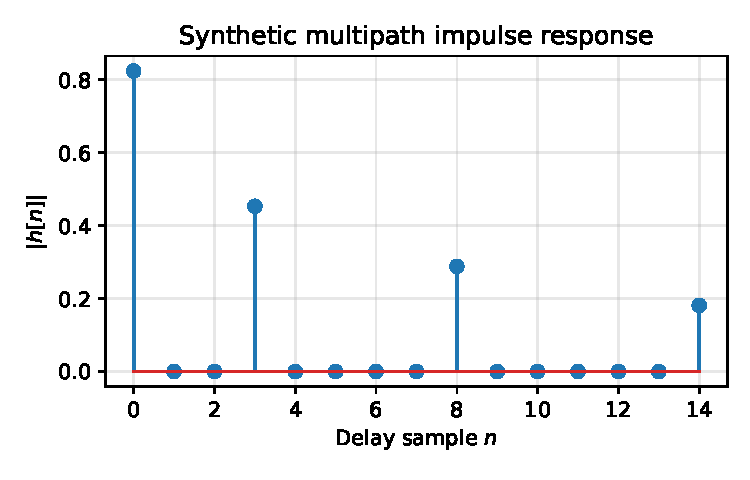
\includegraphics[width=\columnwidth]{channel_impulse_response.pdf}
    \caption{Synthetic multipath channel impulse response. The largest nonzero delay is 14 samples, so a 16-sample cyclic prefix can absorb the delay spread.}
    \label{fig:channel-impulse}
\end{figure}

\begin{figure}[!t]
    \centering
    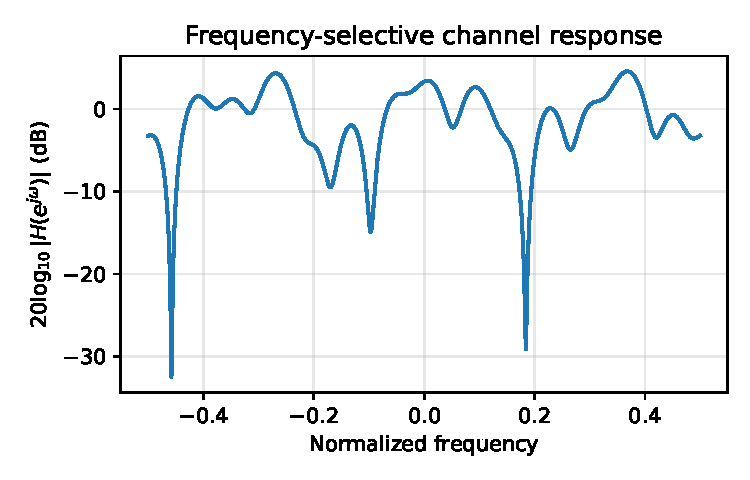
\includegraphics[width=\columnwidth]{channel_frequency_response.pdf}
    \caption{Frequency response of the synthetic multipath channel. Frequency-selective gains motivate subcarrier-by-subcarrier equalization.}
    \label{fig:channel-frequency}
\end{figure}

\begin{figure}[!t]
    \centering
    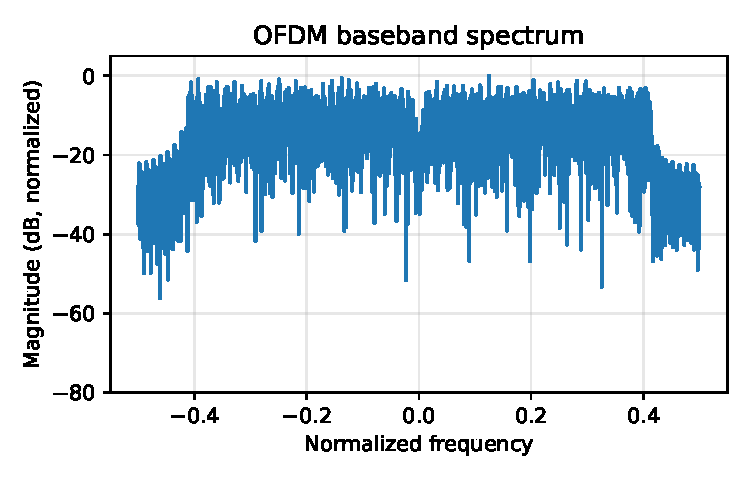
\includegraphics[width=\columnwidth]{ofdm_spectrum.pdf}
    \caption{Spectrum of a generated OFDM baseband signal. The DC bin and guard bins are left unused.}
    \label{fig:ofdm-spectrum}
\end{figure}

\subsection{When Does the One-Tap OFDM Model Become Valid?}
Fig.~\ref{fig:cp-error} directly tests the mathematical claim behind OFDM equalization. For a single OFDM block, the code compares the actual DFT-domain output to the ideal model $Y[k]=H[k]X[k]$. When the cyclic prefix is shorter than $L-1$, the model is not exact because the channel convolution leaks between blocks. Once $N_{cp}\geq L-1$, the relative error drops to numerical precision in the noiseless test. This connects the project directly to the class result that convolution becomes multiplication after a Fourier transform, with the added condition that OFDM needs circular rather than linear convolution.

\begin{figure}[!t]
    \centering
    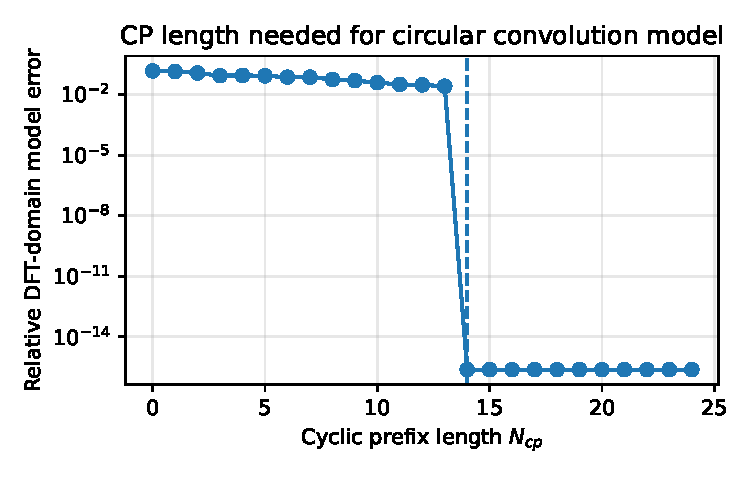
\includegraphics[width=\columnwidth]{cyclic_prefix_error.pdf}
    \caption{Relative error between the actual DFT-domain output and the ideal one-tap model $Y[k]=H[k]X[k]$ as a function of cyclic-prefix length. The dashed line marks $L-1$.}
    \label{fig:cp-error}
\end{figure}

\subsection{Cyclic-Prefix Length and Rate Tradeoff}
The key design lesson is that the cyclic prefix helps only until it covers the channel memory; after that point, extra prefix samples mostly reduce rate. Fig.~\ref{fig:cp-sweep} turns the same condition into a BER design experiment at 18 dB SNR. With no cyclic prefix, the mean BER is $8.17\times 10^{-3}$. As $N_{cp}$ approaches the channel memory, the BER falls; at $N_{cp}=14=L-1$ it is $1.66\times 10^{-3}$, and increasing the prefix beyond this point gives little additional improvement for this channel. 

The cost is rate: with 52 active BPSK subcarriers and $N=64$, $R_{\mathrm{eff}}$ decreases from $0.8125$ bits/sample at $N_{cp}=0$ to $0.65$ bits/sample at $N_{cp}=16$ and $0.591$ bits/sample at $N_{cp}=24$. This is the main engineering tradeoff of the cyclic prefix and the clearest acoustic-channel design lesson in the project: robustness improves only until the prefix covers the channel memory, while every additional prefix sample reduces useful throughput.

\begin{figure}[!t]
    \centering
    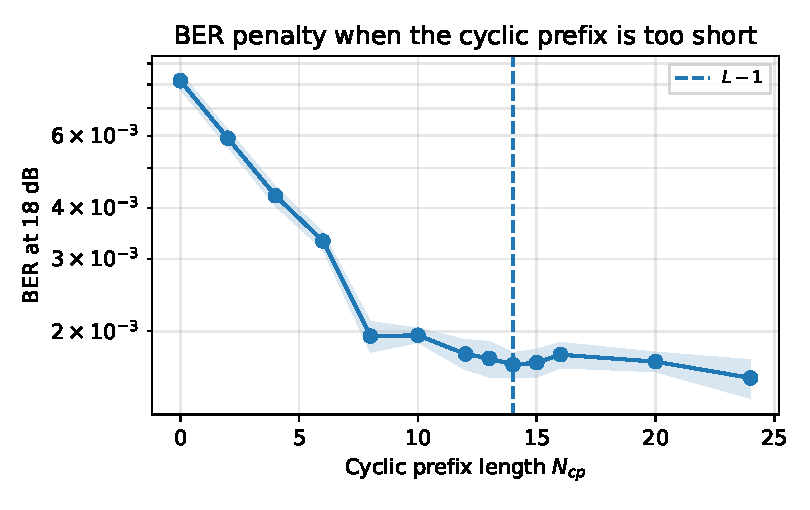
\includegraphics[width=\columnwidth]{cp_length_ber_sweep.pdf}
    \caption{Mean BER at 18 dB versus cyclic-prefix length. BER drops as the prefix approaches the channel memory, but additional prefix length gives little improvement after the dashed line $N_{cp}=L-1$. The shaded band is an approximate 95\% Monte Carlo interval.}
    \label{fig:cp-sweep}
\end{figure}

\subsection{Reliability Under Multipath and Noise}
Fig.~\ref{fig:ber} shows the main packet-recovery result. At low SNR, all schemes are limited by noise. At moderate and high SNR, the OFDM curves separate according to whether the receiver has a valid circular-convolution model and a channel equalizer. The single-carrier matched filter performs well in pure AWGN, but it has a large error floor in the echo-rich multipath test because the receiver has no equalizer and therefore cannot remove ISI.


\begin{figure}[!t]
    \centering
    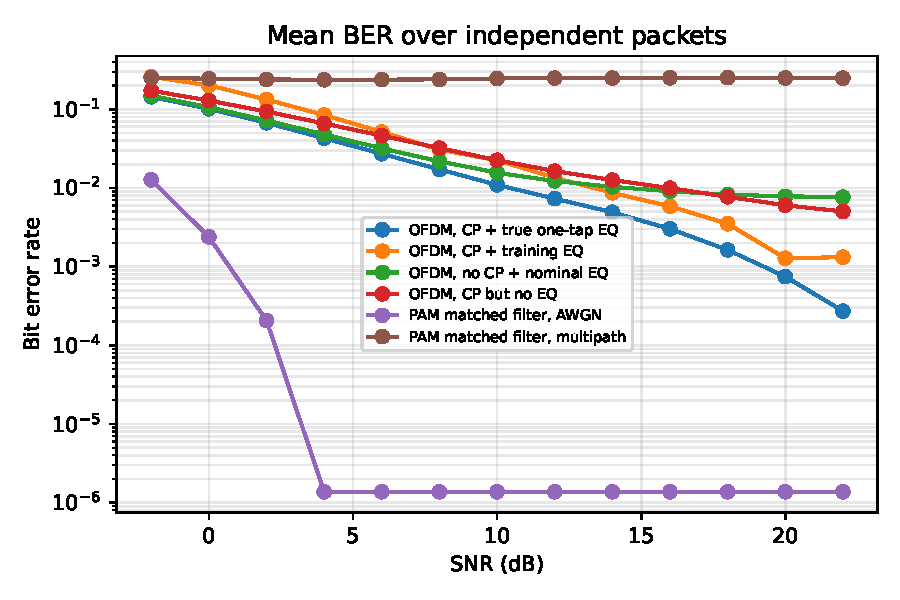
\includegraphics[width=\columnwidth]{ber_curves.pdf}
    \caption{Mean bit error rate versus SNR over 20 independent packet trials. CP-OFDM with one-tap equalization improves with SNR, while single-carrier matched filtering without equalization has an ISI-driven error floor in the multipath channel.}
    \label{fig:ber}
\end{figure}

\begin{table}[!t]
    \caption{Monte Carlo BER Values, Mean $\pm$ Approximate 95\% CI, in $10^{-3}$}
    \label{tab:ber}
    \centering
    \scriptsize
    \begin{tabular}{lcc}
        \toprule
        Receiver & 12 dB & 18 dB\\
        \midrule
        OFDM, CP + true EQ & $7.31\!\pm\!0.27$ & $1.63\!\pm\!0.11$\\
        OFDM, CP + training EQ & $13.51\!\pm\!2.07$ & $3.51\!\pm\!1.31$\\
        OFDM, no CP + nominal EQ & $12.26\!\pm\!0.32$ & $8.20\!\pm\!0.25$\\
        OFDM, CP but no EQ & $16.37\!\pm\!0.31$ & $7.73\!\pm\!0.20$\\
        PAM matched filter, AWGN & $0$ obs. & $0$ obs.\\
        PAM matched filter, multipath & $249.1\!\pm\!1.5$ & $252.0\!\pm\!1.9$\\
        \bottomrule
    \end{tabular}
\end{table}

Table~\ref{tab:ber} shows that the training-symbol equalizer has a visible penalty at low and moderate SNR because $\hat{H}[k]$ is itself noisy. The true-channel equalizer therefore gives the best CP-OFDM curve, as expected. The no-CP and no-equalizer cases have comparable high-SNR BERs for this particular channel, but for different reasons: without a cyclic prefix the one-tap model is invalid, while without equalization the channel rotation and frequency-selective attenuation are left in the constellation. The zero entries for PAM in AWGN mean that no bit errors were observed in the simulated finite run, not that the theoretical BER is exactly zero.

Taken together, these results suggest three design lessons for acoustic OFDM links. First, the cyclic prefix should be chosen based on the measured or estimated channel memory rather than increased arbitrarily. Second, frequency-domain equalization is only meaningful when the cyclic prefix is long enough for the one-tap subcarrier model to be approximately valid. Third, training-based channel estimates introduce their own reliability penalty at low SNR, so practical systems must balance overhead, estimation quality, and throughput.

\subsection{What the Equalizer Does to the Subcarriers}
Fig.~\ref{fig:constellation-before} and Fig.~\ref{fig:constellation-after} show the received subcarrier symbols before and after equalization. Before equalization, each subcarrier has been scaled and rotated by the channel response. After dividing by $H[k]$, the points cluster again near the BPSK decision regions. This visualization is a compact way to show what the frequency-domain equalizer is doing: it turns a frequency-selective acoustic channel from a collection of rotated, attenuated subcarriers back into approximately common BPSK decision regions.

\begin{figure}[!t]
    \centering
    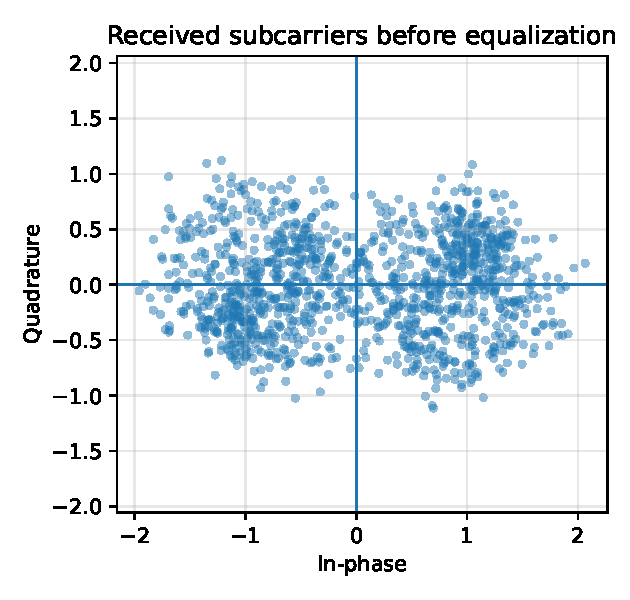
\includegraphics[width=0.9\columnwidth]{constellation_before_equalization.pdf}
    \caption{Received active-subcarrier values before equalization. The multipath channel scales and rotates the symbols differently across frequency.}
    \label{fig:constellation-before}
\end{figure}

\begin{figure}[!t]
    \centering
    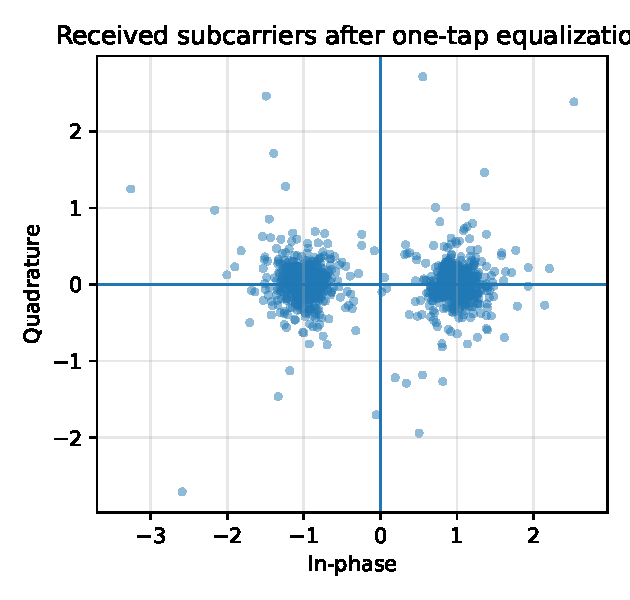
\includegraphics[width=0.9\columnwidth]{constellation_after_equalization.pdf}
    \caption{Received active-subcarrier values after one-tap equalization. The symbols return to the expected decision regions.}
    \label{fig:constellation-after}
\end{figure}

\section{Part III: From Complex Baseband to Real-Valued Audio Packets}

\subsection{Real-Valued Audio OFDM}
The synthetic OFDM experiment uses complex baseband signals. A real speaker, however, plays a real-valued waveform. The audio extension therefore uses Hermitian DFT symmetry. This symmetry is needed because arbitrary complex frequency bins usually produce a complex IFFT output, while a speaker can only play a real-valued waveform. If positive-frequency bins contain symbols $X[k]$, the negative-frequency bins are set to
\begin{equation}
    X[N-k]=X^*[k].
\end{equation}
This makes the IFFT output real. The demo uses active positive-frequency bins from 16 to 64 of a 256-point IFFT at 48 kHz, corresponding roughly to 3--12 kHz. A short silence, two repeated preamble OFDM symbols, data symbols, and a final silence are concatenated and written to \texttt{audio/tx\_packet.wav}.

The receiver finds the packet start by correlating the recording with the known preamble. In the implemented normalized detector,
\begin{equation}
    \hat{n}_0=\arg\max_n
    \frac{\left|\sum_{\ell=0}^{P-1}r[n+\ell]p^*_{\mathrm{pre}}[\ell]\right|}
    {\sqrt{\sum_{\ell=0}^{P-1}|r[n+\ell]|^2\sum_{\ell=0}^{P-1}|p_{\mathrm{pre}}[\ell]|^2}},
    \label{eq:preamble-corr}
\end{equation}
where $p_{\mathrm{pre}}$ is the known preamble waveform and $P$ is its length. The receiver then estimates $\hat{H}[k]$ from the last preamble block and decodes the data blocks using \eqref{eq:zf}. In the simulated loopback test, the channel is a bandlimited echo response shorter than the cyclic prefix, the preamble correlation peak is 0.941, and the decoded text is exactly recovered:
\begin{center}
\texttt{ES156 audio OFDM: the FFT diagonalizes a cyclic convolution.}
\end{center}

\begin{figure}[!t]
    \centering
    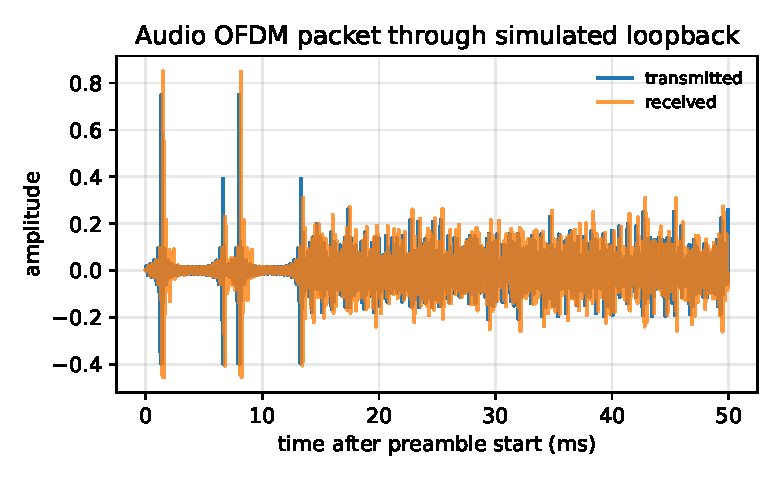
\includegraphics[width=\columnwidth]{audio_loopback_waveform.pdf}
    \caption{Real-valued audio OFDM packet before and after the simulated speaker-room-microphone channel.}
    \label{fig:audio-waveform}
\end{figure}

\begin{figure}[!t]
    \centering
    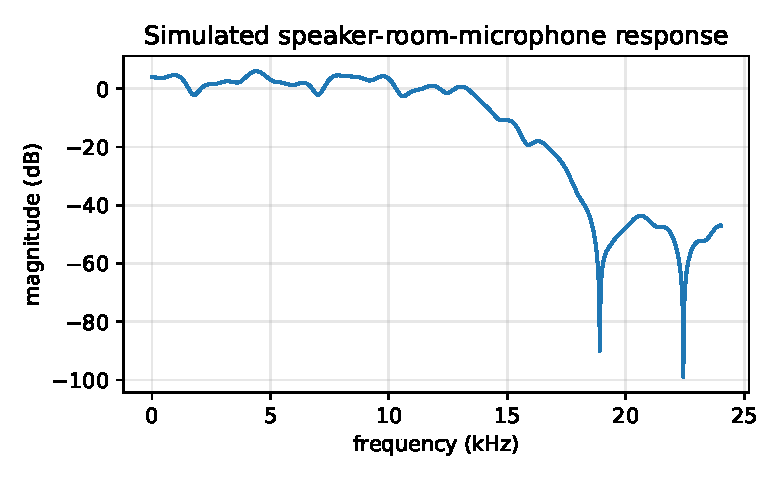
\includegraphics[width=\columnwidth]{audio_loopback_channel_response.pdf}
    \caption{Frequency response of the simulated audio loopback channel used in the WAV-packet experiment.}
    \label{fig:audio-channel}
\end{figure}

\subsection{Passband Sanity Check}
A second optional script implements a conventional passband loopback. It modulates a smaller complex-baseband OFDM signal onto an 8 kHz real carrier, applies a simulated acoustic echo channel, mixes the received signal back down, low-pass filters it, estimates the channel from one training OFDM symbol, and decodes the message. Fig.~\ref{fig:passband-spectrum} shows that the generated signal occupies an audio band around the carrier. This script is not used for the main BER curves because it assumes the packet start is known, but it is a useful check that the same FFT-equalization idea can be embedded in a real-valued audio waveform. The decoded passband-loopback message has BER $0$ in the included reproducible run.

\begin{figure}[!t]
    \centering
    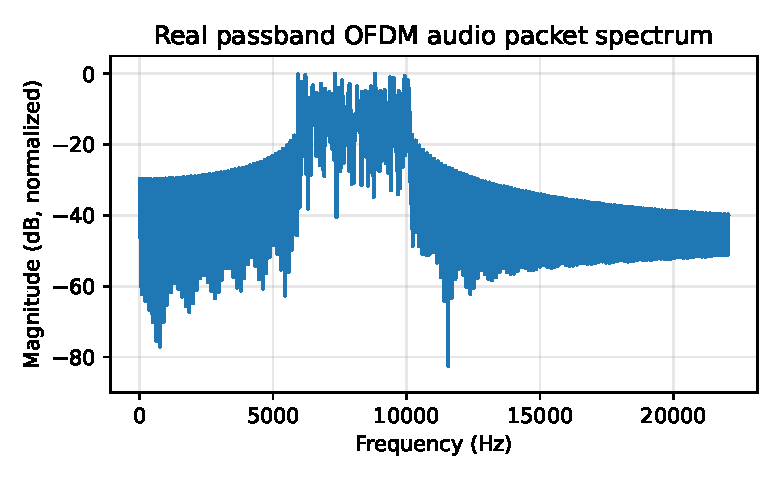
\includegraphics[width=\columnwidth]{passband_audio_spectrum.pdf}
    \caption{Spectrum of the optional real passband OFDM audio packet centered near 8 kHz.}
    \label{fig:passband-spectrum}
\end{figure}

\subsection{Gap to Real Room-Acoustic and Sonar Channels}

This framework deliberately simplifies real underwater and over-the-air acoustic channels. The synthetic channel is static, finite-length, and exactly known in some experiments; it omits Doppler spread, time-varying multipath, transducer nonlinearities, automatic gain control, sample-rate mismatch, and environmental propagation effects. The goal is educational and experimental reproducibility: to isolate the cyclic-prefix and FFT-equalization mechanism under controlled conditions, rather than to claim deployment-grade underwater modem performance.

The synthetic and simulated loopback experiments isolate the core OFDM mechanism: a cyclic prefix converts the channel convolution into an approximately circular convolution, after which FFT-domain equalization reduces to scalar division on each active subcarrier. This makes the project useful as an acoustic-channel testbed, but several effects separate it from a true underwater modem or measured over-the-air speaker-microphone link.

First, the receiver would not know the packet start time a priori. The preamble detector in \eqref{eq:preamble-corr} is a first step, but a practical system would need more robust timing acquisition and tracking. Small timing errors within the cyclic-prefix tolerance may be absorbed by the channel estimate, but timing errors outside this region destroy subcarrier orthogonality and introduce ISI and intercarrier interference (ICI).

Second, real rooms and underwater channels generally have denser and longer impulse responses than the four-path synthetic channel used in the baseline experiment. Early reflections and a decaying reverberation tail can leave significant delayed energy beyond the cyclic prefix. In that case, the one-tap model $Y[k]=H[k]X[k]+W[k]$ no longer holds exactly, and the receiver can develop a high-SNR error floor, meaning that the error rate stops improving even when more noise is removed. This is why the cyclic-prefix-length sweep is the most important experiment: it exposes the boundary between a valid OFDM subchannel model and a channel whose delay spread is too long for the chosen prefix.

Third, underwater links introduce Doppler and time variation much more strongly than the static channel used here. Real playback and recording devices may also introduce frequency offset, sample-rate mismatch, and slow timing drift. These effects can rotate constellations, shift subcarriers, and create ICI. A robust acoustic modem would therefore require frequency-offset estimation and timing tracking in addition to one-tap equalization.

Finally, speaker and microphone responses were not separately modeled. Their approximately linear frequency responses could be absorbed into the estimated channel response $\hat{H}[k]$, but nonlinear effects such as clipping, automatic gain control, and loudspeaker distortion would not be removed by one-tap equalization. Real environmental noise may also be colored, impulsive, or narrowband rather than white and Gaussian.

\section{Conclusion}
This project reframed acoustic data transmission around a single design question: when does cyclic-prefix OFDM make a dispersive acoustic channel behave like independent FFT subchannels? The single-carrier PAM baseline demonstrates matched filtering and threshold detection, while also showing the high-SNR ISI floor that appears when a receiver has no equalizer. The OFDM system demonstrates the power of the DFT for converting convolution into multiplication, provided the cyclic prefix is long enough to make the useful block look circular.

The results support three conclusions. First, the cyclic prefix is not just overhead; it is the condition that makes the one-tap equalizer mathematically valid. Second, FFT-domain equalization substantially lowers BER in the tested multipath channel compared with OFDM without a valid cyclic-prefix model or OFDM without equalization. Third, the prefix length creates a measurable rate/robustness tradeoff: performance improves when the prefix reaches the channel memory, but every extra sample reduces useful data rate. The simulated real-valued audio extension shows that the same idea can be packaged as a synchronized WAV packet, making the framework a small but complete acoustic-communication testbed.

The project is intentionally narrower than a full underwater or commodity-device acoustic modem. It does not solve Doppler, mobility, real-room calibration, coding, or adaptive synchronization. Future work could measure a real room impulse response using a swept sine \cite{farina2000}, record the packet through an actual speaker and microphone, compare zero-forcing and MMSE equalization in deep spectral nulls, add frequency-offset correction, and test QPSK or 16-QAM with forward error correction. These extensions would move the testbed closer to practical acoustic networking while preserving the core signals-and-systems focus on convolution, Fourier analysis, sampling, synchronization, and filtering.

\section*{Code Availability}
All code for the synthetic experiments and audio demonstrations is organized as a small Python project and is available in the GitHub repository
\href{https://github.com/Giancarla-Burgos/ES156_Final_Project}{Giancarla-Burgos/ES156\_Final\_Project}.

The repository README lists the Python dependencies, the fixed random-number settings used to make the simulations reproducible, the purpose of each script, the expected output folders, and the commands needed to regenerate the figures and CSV summaries. The main reproducibility commands are

\begingroup\scriptsize\begin{verbatim}
python3 scripts/run_experiments.py
python3 scripts/run_audio_loopback_demo.py
python3 scripts/run_passband_audio_loopback.py
python3 scripts/make_audio_packet.py
python3 scripts/decode_recorded_packet.py \
    audio/recorded_packet.wav
\end{verbatim}\endgroup
The generated figures, CSV summaries, and optional WAV files are saved in \texttt{figures/}, \texttt{results/}, and \texttt{audio/}, respectively.

Thus, the main BER curves, cyclic-prefix sweep, constellation plots, channel plots, and audio-loopback outputs can be regenerated from the scripts rather than manually assembled.

\begin{thebibliography}{99}

\bibitem{oppenheim1997}
A.~V. Oppenheim, A.~S. Willsky, and S.~H. Nawab, \emph{Signals and Systems}, 2nd~ed. Upper Saddle River, NJ, USA: Prentice Hall, 1997.

\bibitem{proakis2008}
J.~G. Proakis and M.~Salehi, \emph{Digital Communications}, 5th~ed. New York, NY, USA: McGraw-Hill, 2008.

\bibitem{weinstein1971}
S.~B. Weinstein and P.~M. Ebert, ``Data transmission by frequency-division multiplexing using the discrete Fourier transform,'' \emph{IEEE Transactions on Communication Technology}, vol.~19, no.~5, pp.~628--634, 1971.

\bibitem{bingham1990}
J.~A.~C. Bingham, ``Multicarrier modulation for data transmission: An idea whose time has come,'' \emph{IEEE Communications Magazine}, vol.~28, no.~5, pp.~5--14, 1990.

\bibitem{nee2000}
R.~van Nee and R.~Prasad, \emph{OFDM for Wireless Multimedia Communications}. Boston, MA, USA: Artech House, 2000.

\bibitem{schmidl1997}
T.~M. Schmidl and D.~C. Cox, ``Robust frequency and timing synchronization for OFDM,'' \emph{IEEE Transactions on Communications}, vol.~45, no.~12, pp.~1613--1621, 1997.

\bibitem{farina2000}
A.~Farina, ``Simultaneous measurement of impulse response and distortion with a swept-sine technique,'' presented at the 108th Audio Engineering Society Convention, Paris, France, 2000.


\bibitem{stojanovic2008}
M.~Stojanovic, ``OFDM for underwater acoustic communications: Adaptive synchronization and sparse channel estimation,'' in \emph{Proc. IEEE International Conference on Acoustics, Speech and Signal Processing (ICASSP)}, 2008, pp.~5288--5291.

\bibitem{feng2023}
C.~Feng, Y.~Luo, J.~Zhang, and H.~Li,
``An OFDM-based frequency domain equalization algorithm for underwater acoustic communication with a high channel utilization rate,''
\emph{Journal of Marine Science and Engineering}, vol.~11, no.~2, art.~415, 2023.

\bibitem{matsuoka2006}
H.~Matsuoka, Y.~Nakashima, and T.~Yoshimura, ``Acoustic communication system using mobile terminal microphones,'' \emph{NTT DoCoMo Technical Journal}, vol.~8, no.~2, pp.~4--12, 2006.

\bibitem{tabak2021}
G.~Tabak, X.~E. Lin, and A.~C. Singer, ``High data rate near-ultrasonic communication with consumer devices,'' in \emph{Proc. European Signal Processing Conference (EUSIPCO)}, 2021, pp.~1681--1685.

\bibitem{wang2016}
Q.~Wang, K.~Ren, M.~Zhou, T.~Lei, D.~Koutsonikolas, and L.~Su, ``Messages behind the sound: Real-time hidden acoustic signal capture with smartphones,'' in \emph{Proc. ACM MobiCom}, 2016, pp.~29--41.

\end{thebibliography}

\end{document}
